\documentclass{sicp}

\geometry{a3paper, margin={1in}}

\date{August 17, 2024}

\begin{document}

\maketitle

\sicptext{
	Draw the tree illustrating the process generated by the \texttt{count-change} procedure of 1.2.2 in making change for 11 cents. What are the orders of growth of the space and number of steps used by this process as the amount to be changed increases?
}

Well, I've always wanted to try my hand at TikZ (\texttt{first-denomination} abbreviated to \texttt{fd}):

\begin{figure}[hbtp]
	\centering
	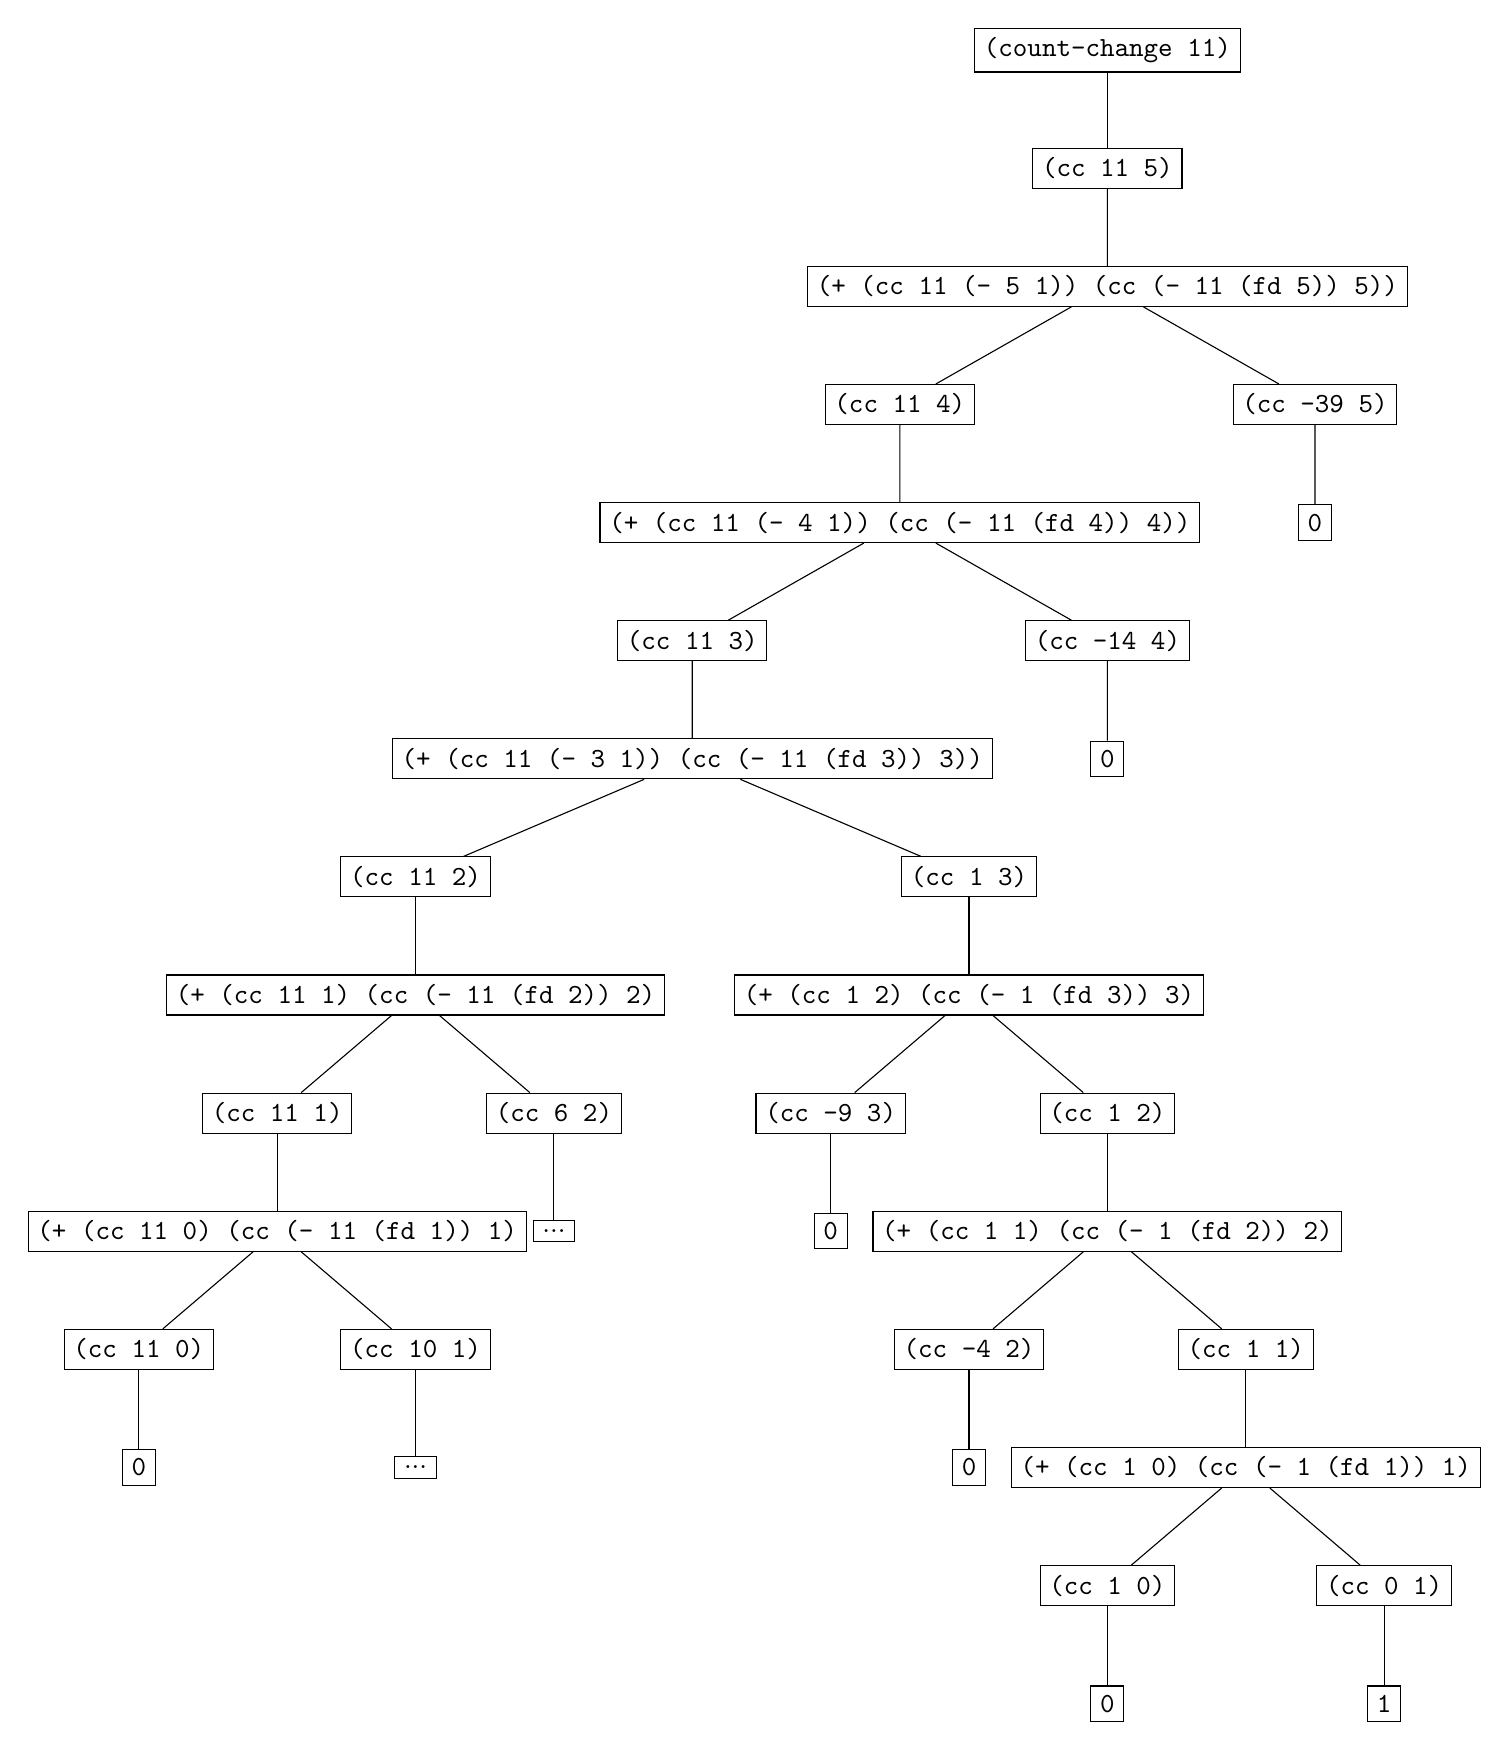
\begin{tikzpicture}[node distance=5mm and 5mm, every node/.style={draw,rectangle,align=center}, level 3/.style={sibling distance=15em}, level 7/.style={sibling distance=20em}]
		\node {\texttt{(count-change 11)}}
		child {node {\texttt{(cc 11 5)}}
				child {node {\texttt{(+ (cc 11 (- 5 1)) (cc (- 11 (fd 5)) 5))}}
						child {node {\texttt{(cc 11 4)}}
								child {node {\texttt{(+ (cc 11 (- 4 1)) (cc (- 11 (fd 4)) 4))}}
										child {node {\texttt{(cc 11 3)}}
												child {node {\texttt{(+ (cc 11 (- 3 1)) (cc (- 11 (fd 3)) 3))}}
														child {node {\texttt{(cc 11 2)}} [sibling distance=10em]
																child {node {\texttt{(+ (cc 11 1) (cc (- 11 (fd 2)) 2)}}
																		child {node {\texttt{(cc 11 1)}}
																				child {node {\texttt{(+ (cc 11 0) (cc (- 11 (fd 1)) 1)}}
																						child {node {\texttt{(cc 11 0)}}
																								child {node {\texttt{0}}}
																							}
																						child {node {\texttt{(cc 10 1)}}
																								child {node {...}}
																							}
																					}
																			}
																		child {node {\texttt{(cc 6 2)}}
																				child {node {...}}
																			}
																	}
															}
														child {node  {\texttt{(cc 1 3)}} [sibling distance=10em]
																child {node {\texttt{(+ (cc 1 2) (cc (- 1 (fd 3)) 3)}}
																		child {node {\texttt{(cc -9 3)}}
																				child {node {\texttt{0}}
																					}}
																		child {node {\texttt{(cc 1 2)}}
																				child {node {\texttt{(+ (cc 1 1) (cc (- 1 (fd 2)) 2)}}
																						child {node {\texttt{(cc -4 2)}}
																								child {node {\texttt{0}}}
																							}
																						child {node {\texttt{(cc 1 1)}}
																								child {node {\texttt{(+ (cc 1 0) (cc (- 1 (fd 1)) 1)}}
																										child {node {\texttt{(cc 1 0)}}
																												child {node {\texttt{0}}}
																											}
																										child {node {\texttt{(cc 0 1)}}
																												child {node {\texttt{1}}}
																											}
																									}}
																					}
																			}
																	}}
													}
											}
										child {node {\texttt{(cc -14 4)}}
												child {node {\texttt{0}}}}
									}}
						child {node {\texttt{(cc -39 5)}}
								child {node {\texttt{0}}
									}}
					}}
		;
	\end{tikzpicture}
\end{figure}

Okay, I've tried my hand at TikZ and it's kind of annoying to deal with a tree this deep now, so I've stopped at the ellipses.

Space requirements here should be $\Theta(n)$, while time is $\Theta(2^n)$, but I'm unsure about this---SICP doesn't elaborate too much on how to determine this, and the CS courses I did about this topic are 5 years in the past at this point.

Well, cross-checking agaisnt what Eli Bendersky wrote, time complexity is actually \emph{not} exponential, despite how it appears.
Instead, the time complexity is on the order of $\Theta(n^5)$ (where the 5 comes from the number of available coins).

\end{document}
